% --- ORIGINAL CONTENT ---
\subsection*{Anderson acceleration: convergence and diagnostics}
\label{subsec:anderson}
\paragraph{Motivation and scope}
To reduce the number of block fixed-point (block Picard/Gauss--Seidel) sub-iterations, we employ Anderson acceleration (AA) with finite memory $m$ in the Walker--Ni formulation described in \S\ref{sec:fp-aa}. We compare (i) a block Picard baseline (constant relaxation) and (ii) AA with step limiting and adaptive history restarts across representative couplings and time-step sizes $\Delta t$. We also report diagnostics that help choose~$m$ and monitor robustness.

\subsection*{Projected residual and stopping}\label{subsec:proj_merit}
We use the \emph{RMS-per-DOF} Picard residual $r_{\mathrm{Pic}}$ in \eqref{eq:fp-picard-res} on the flattened state $(\mathbf L,S,\rho)$ with the per-block scaling \eqref{eq:fp-scales}. The coupled solve stops when $r_{\mathrm{Pic}}\le \mathrm{tol}$ or when the maximum number of subiterations is reached. There is no per-iteration AA rejection/backtracking; robustness is provided by the step limiter \eqref{eq:aa-step-limit} and by history restarts based on conditioning and stall. Candidate formation follows \eqref{eq:aa-weights}--\eqref{eq:aa-update}.

\subsection*{Stacking vs.\ sweep order}\label{subsec:order}
The accelerated stacked state follows $(\mathbf L,S,\rho)$, while a single GS sweep updates blocks in the physical order \emph{mechanics driver} $\to$ fabric $\to$ stimulus $\to$ density (mechanics is recomputed inside the driver and is not part of the Anderson state).

\subsection*{Anderson acceleration details}\label{subsec:aa_details}
We employ the Walker--Ni Anderson scheme described in \S\ref{sec:fp-aa}. Specific settings for the results below include the step limit factor $c_{\mathrm{step}}$ and history depths $m$ as indicated in the figures. We restart the AA history upon (i) stagnation of $r_{\mathrm{Pic}}$ relative to the best value in a recent window, or (ii) poor conditioning of the regularized Gram system.

\paragraph{Performance diagnostics}
To assess stability and tuning, we monitor Anderson metrics over time and their sensitivity to $(\Delta t, m, \beta)$ (\cref{fig:aa-metrics}). At fixed $\Delta t=25$ days, a sliding-window view of the condition number $\kappa(H+\lambda_{\mathrm{eff}}I)$ remains well behaved across tested histories $m$ and mixing factors $\beta$. Aggregated over late-time windows, the timestep rejection rate stays moderate, the average history depth scales with $m$, and the median $\kappa(H+\lambda_{\mathrm{eff}}I)$ shows only mild growth with larger $m$ or $\beta$.

\begin{figure}[htbp]
  \centering
  \IfFileExists{images/anderson_performance_vs_time.png}{%
    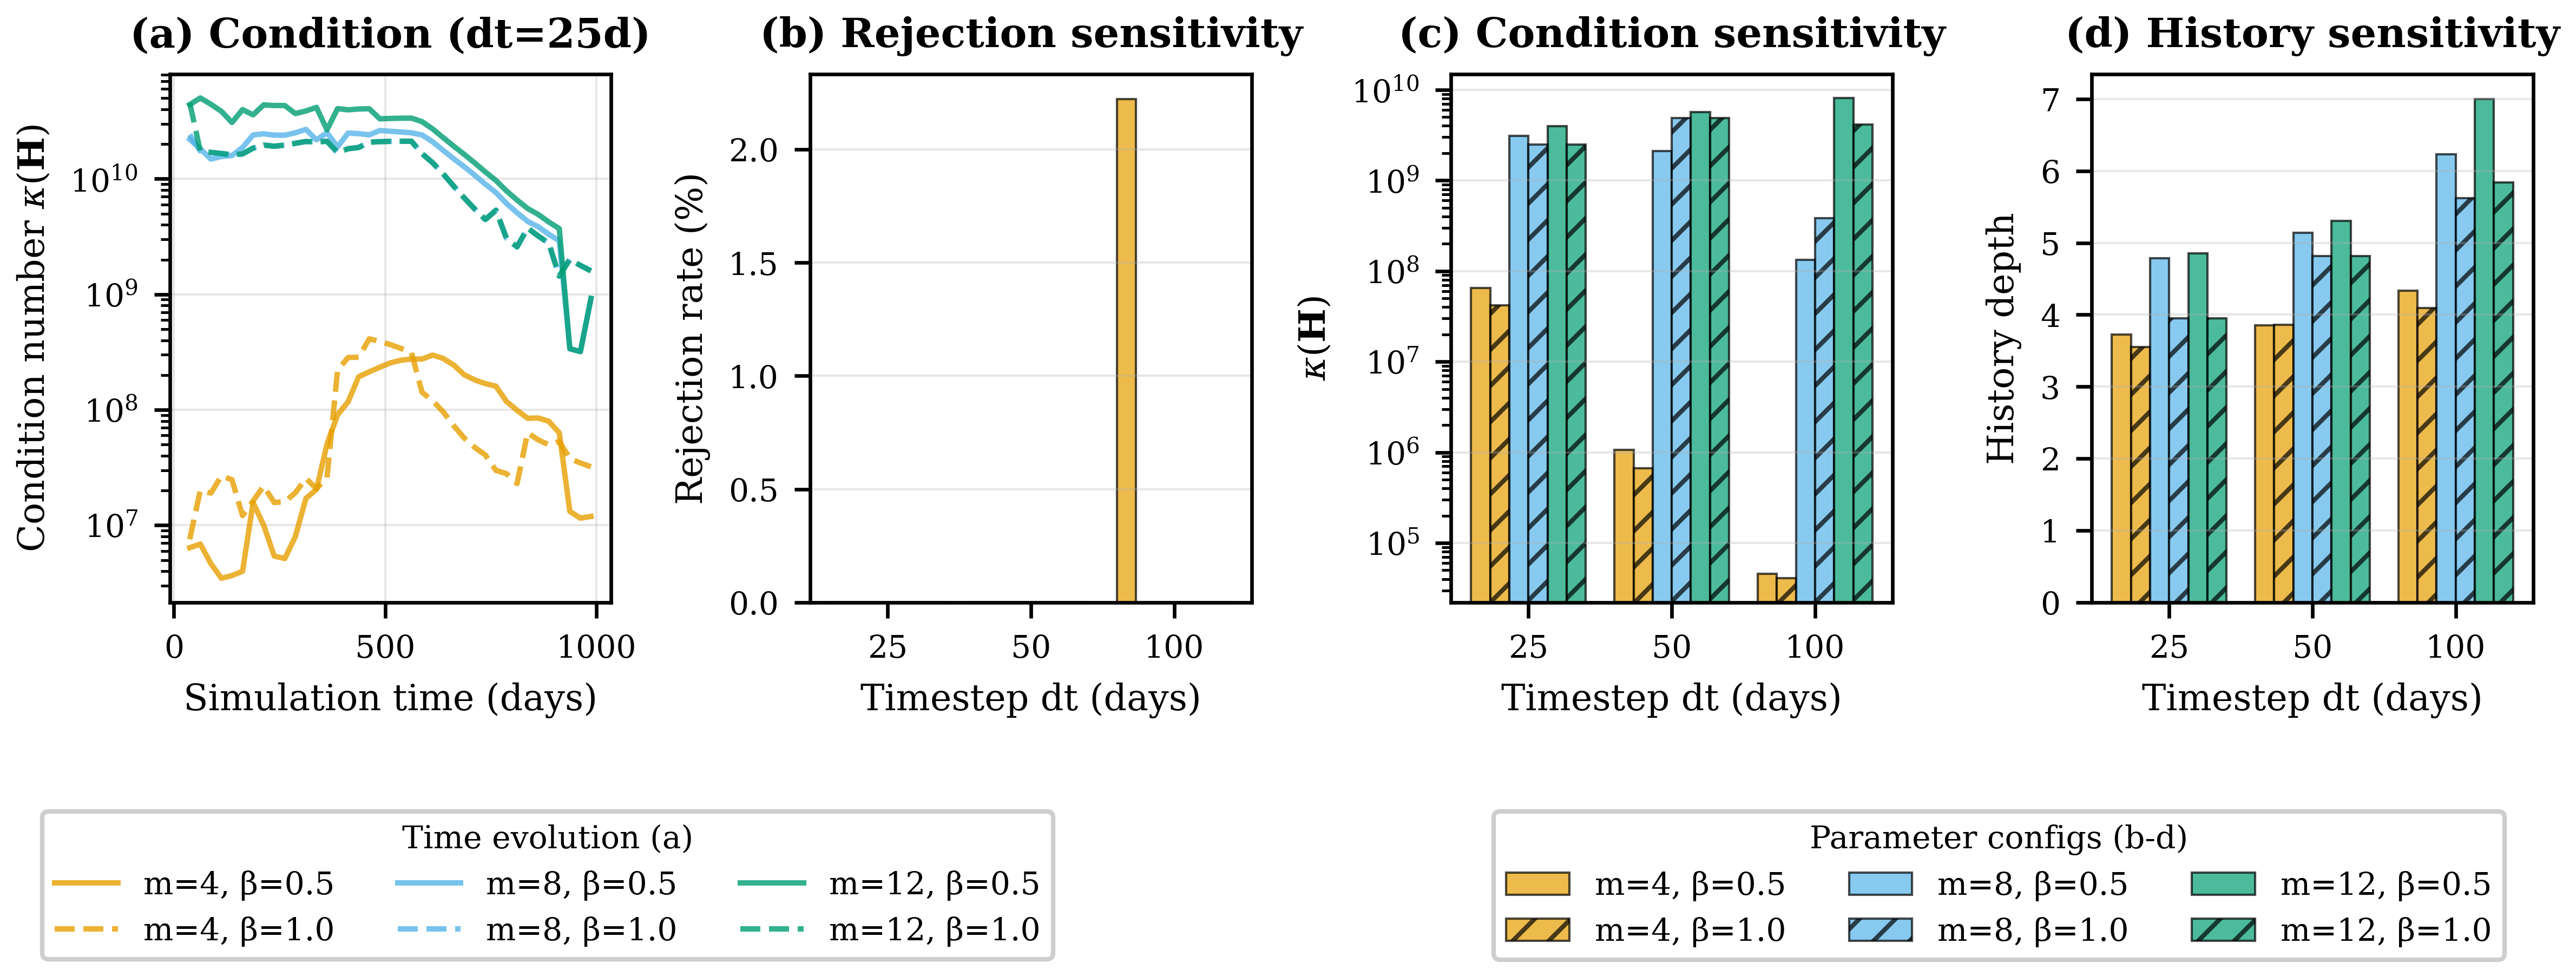
\includegraphics[width=1\linewidth]{images/anderson_performance_vs_time.png}%
  }{\fbox{\parbox{0.9\linewidth}{\centering Missing image: \texttt{images/anderson_performance_vs_time.png}}}}
  \caption{Anderson performance metrics and sensitivity. (a) Time-windowed condition number $\kappa(H+\lambda_{\mathrm{eff}}I)$ at fixed $\Delta t=25$ days for several $(m,\beta)$. (b) Timestep rejection rate (adaptive controller) averaged over the final window versus $\Delta t$, grouped by $(m,\beta)$. (c) Average $\kappa(H+\lambda_{\mathrm{eff}}I)$ (log scale) versus $\Delta t$. (d) Average Anderson history depth versus $\Delta t$.}
  \label{fig:aa-metrics}
\end{figure}

\paragraph{AA vs. Picard}
We compare the baseline block Picard scheme with Anderson acceleration across representative timestep sizes and coupling strengths (\cref{fig:aa-vs-picard}). In our runs, Anderson acceleration reduces sub-iterations per timestep and total walltime while preserving robustness via step limiting and history restarts; the benefit is largest in tighter couplings, with comparable behavior to Picard in mild regimes.

\begin{figure}[htbp]
  \centering
  \IfFileExists{images/anderson_vs_picard.png}{%
    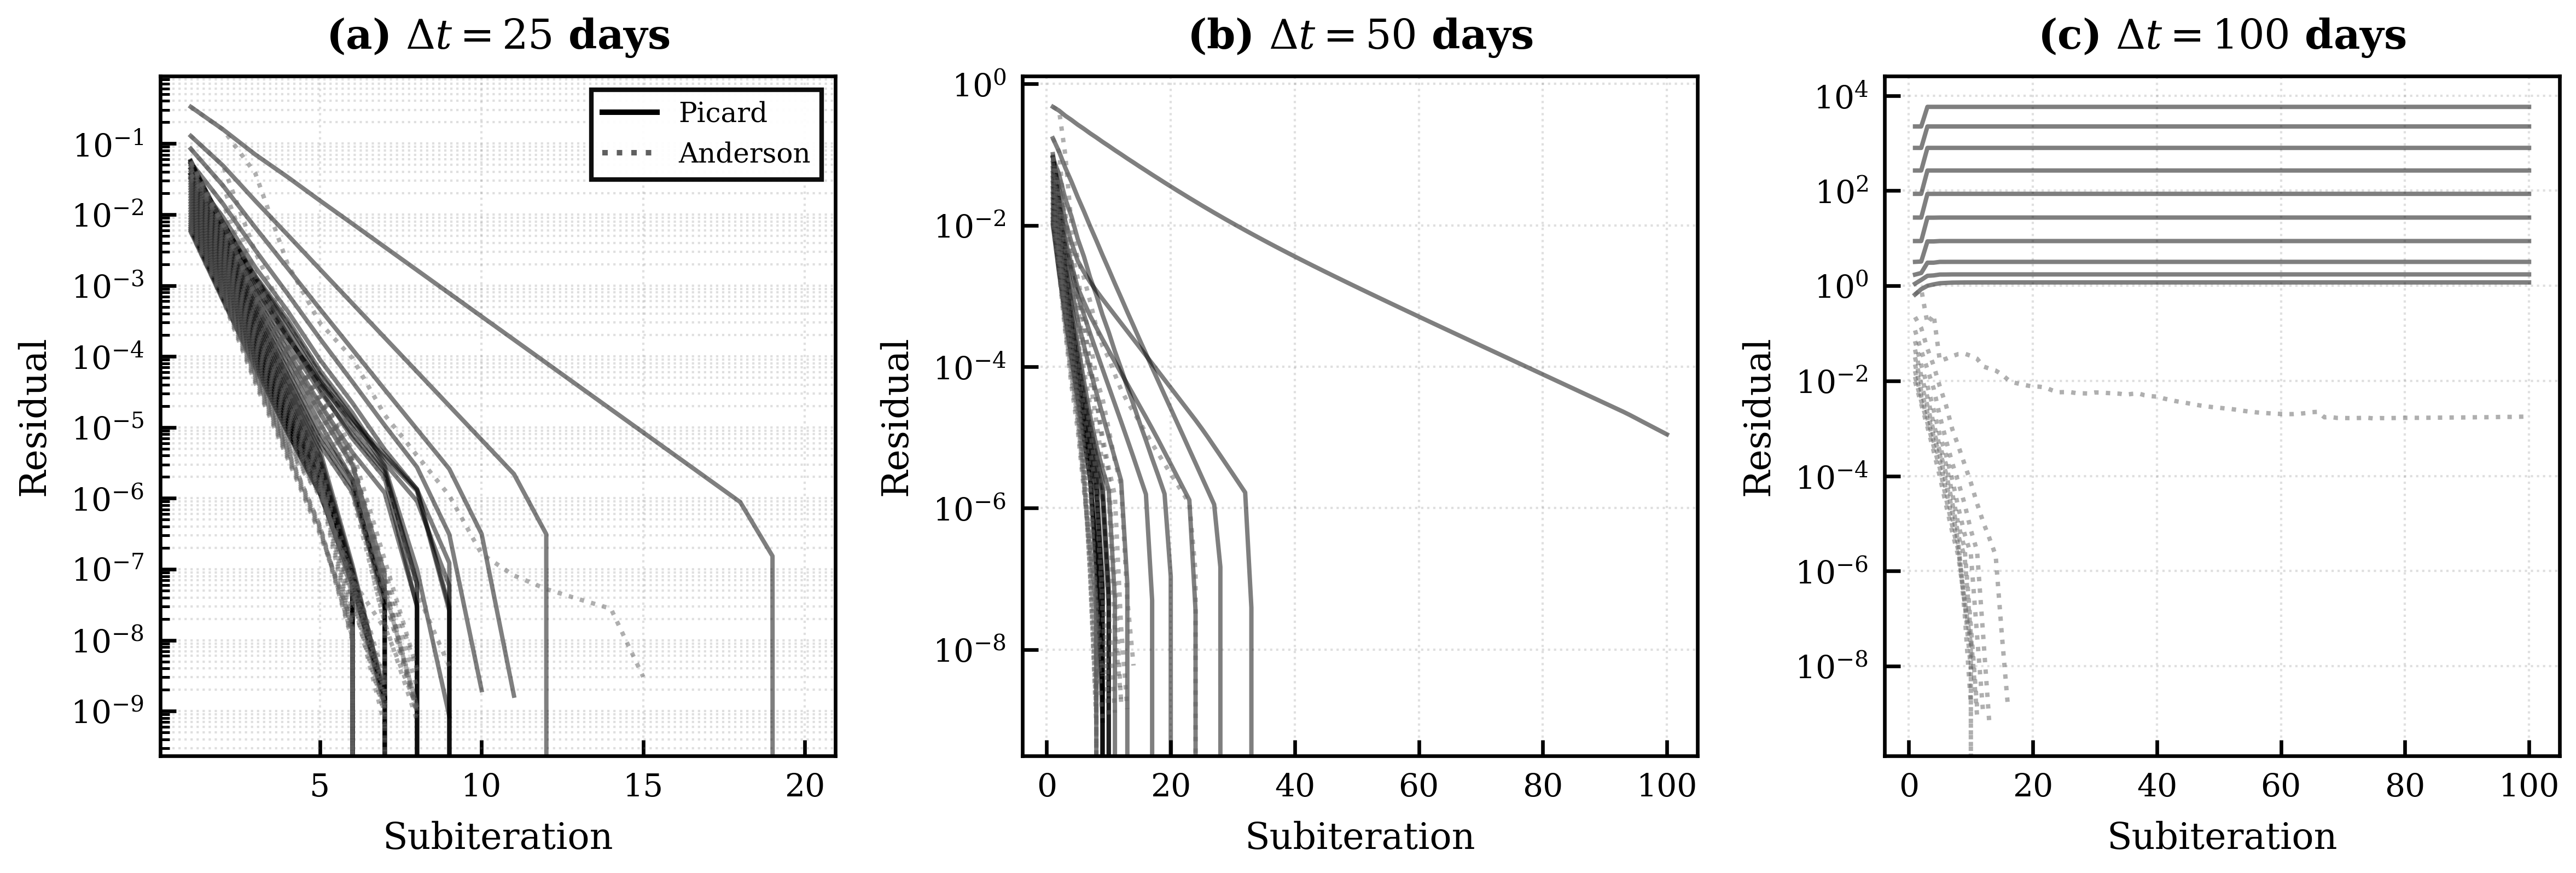
\includegraphics[width=1\linewidth]{images/anderson_vs_picard.png}%
  }{\fbox{\parbox{0.9\linewidth}{\centering Missing image: \texttt{images/anderson_vs_picard.png}}}}
  \caption{Comparison of block Picard and Anderson acceleration at representative $\Delta t$ and coupling strengths. Left: convergence behavior over time (projected-residual trends). Right: per-timestep subiterations and walltime summaries. Anderson acceleration reduces sub-iterations and computational cost while retaining robustness relative to Picard.}
  \label{fig:aa-vs-picard}
\end{figure}
